\chapter{Exercise 1.1}

\section{Problem}

\begin{enumerate}
    \item Imagine an artificial computer language, which can be utilized to solve a practical problem, i.e. the application of the language.
    \begin{itemize}
        \item Tips 1. Language is an alternative approach to problem solving.
        \item Tips 2. First find a proper problem, then design a language to solve the problem.
    \end{itemize}
    \item Give an example of a complete piece written in the proposed language.
    \item Discuss how to define the new language and try your approach.
    \item Describe the process of changing the thinking of your language to a reality, i.e. how to make the artificial language usable.

\end{enumerate}

\section{Solution}

\subsection{Problem 1}

我设计的语言想要解决的问题是实现计算器的某些功能，包括加、减、乘、除、幂、对数和开根号。这种语言所解决的计算均为二元计算，每条语句以运算符开始，后面为两个待计算的数字，以分号结束，并且运算符与两个操作数以“\&”分开，中间可以有随意数量的空格。
运算符（假设第一个数字为a，第二个为b）：
\begin{itemize}
    \item \texttt{+-*/} 分别代表加减乘除；
    \item \texttt{\string^} 代表幂运算，后面第一个为底数，第二个数字为指数，即 $a^b$；
    \item \texttt{\$} 代表对数运算，第一个数为底数，第二个数为真数，即 $\log_a b$；
    \item \texttt{@} 表示开根号，第一个数字为根指数，第二个数为准备开根号的数字，即 $\sqrt[a]{b}$。
\end{itemize}

\subsection{Problem 2}

\begin{lstlisting}
    + & 3 & 5;  //3+5
    * & 2 & 3;  //2*3
    / & 10 & 5; //10/5
    ^ & 2 & 3;  //2的3次方
    $ & 2 & 8;  //以2为低8的对数
    @ & 2 & 4;  //开根号，4的2次方跟，即根号2
\end{lstlisting}

\subsection{Problem 3}

对语言的定义如下：

\begin{itemize}
    \item 字符集：
\end{itemize}

\begin{lstlisting}
{1,2,3,4,5,6,7,8,9,0,+,-,*,/,^,$,@,;}
\end{lstlisting}

\begin{itemize}
    \item BNF：
\end{itemize}

\begin{lstlisting}
<计算语句> ::= <运算符> & integer & integer ;
<运算符> ::= + | - | * | / | ^ | $ | @
integer ::= [ symbol ] unsigned
unsigned ::= digit { digit }
symbol ::= + | -
digit ::= 0 | 1 | ... | 9
\end{lstlisting}

\subsection{Problem 4}

如果想要实现这门语言，当读到指令之后按照 \texttt{\&} 进行分词，先读第一个操作符，针对每种计算分别编写不同的程序，然后读后面的两个操作数，再传给程序计算即可。

\chapter{Exercise 1.2}

\section{Problem}

\begin{enumerate}
    \item Draw a T-diagram with two stages of bootstrappings.
        \begin{itemize}
            \item Given a new programming language L++, we firstly implement L, a small subset of L++.
            \item Then we use L to implement L+, a subset of L++ and a superset of L.
            \item Finally, L++ is implemented using L+.
        \end{itemize}
\end{enumerate}


\section{Solution}

\begin{figure}[htbp]
    \centering
    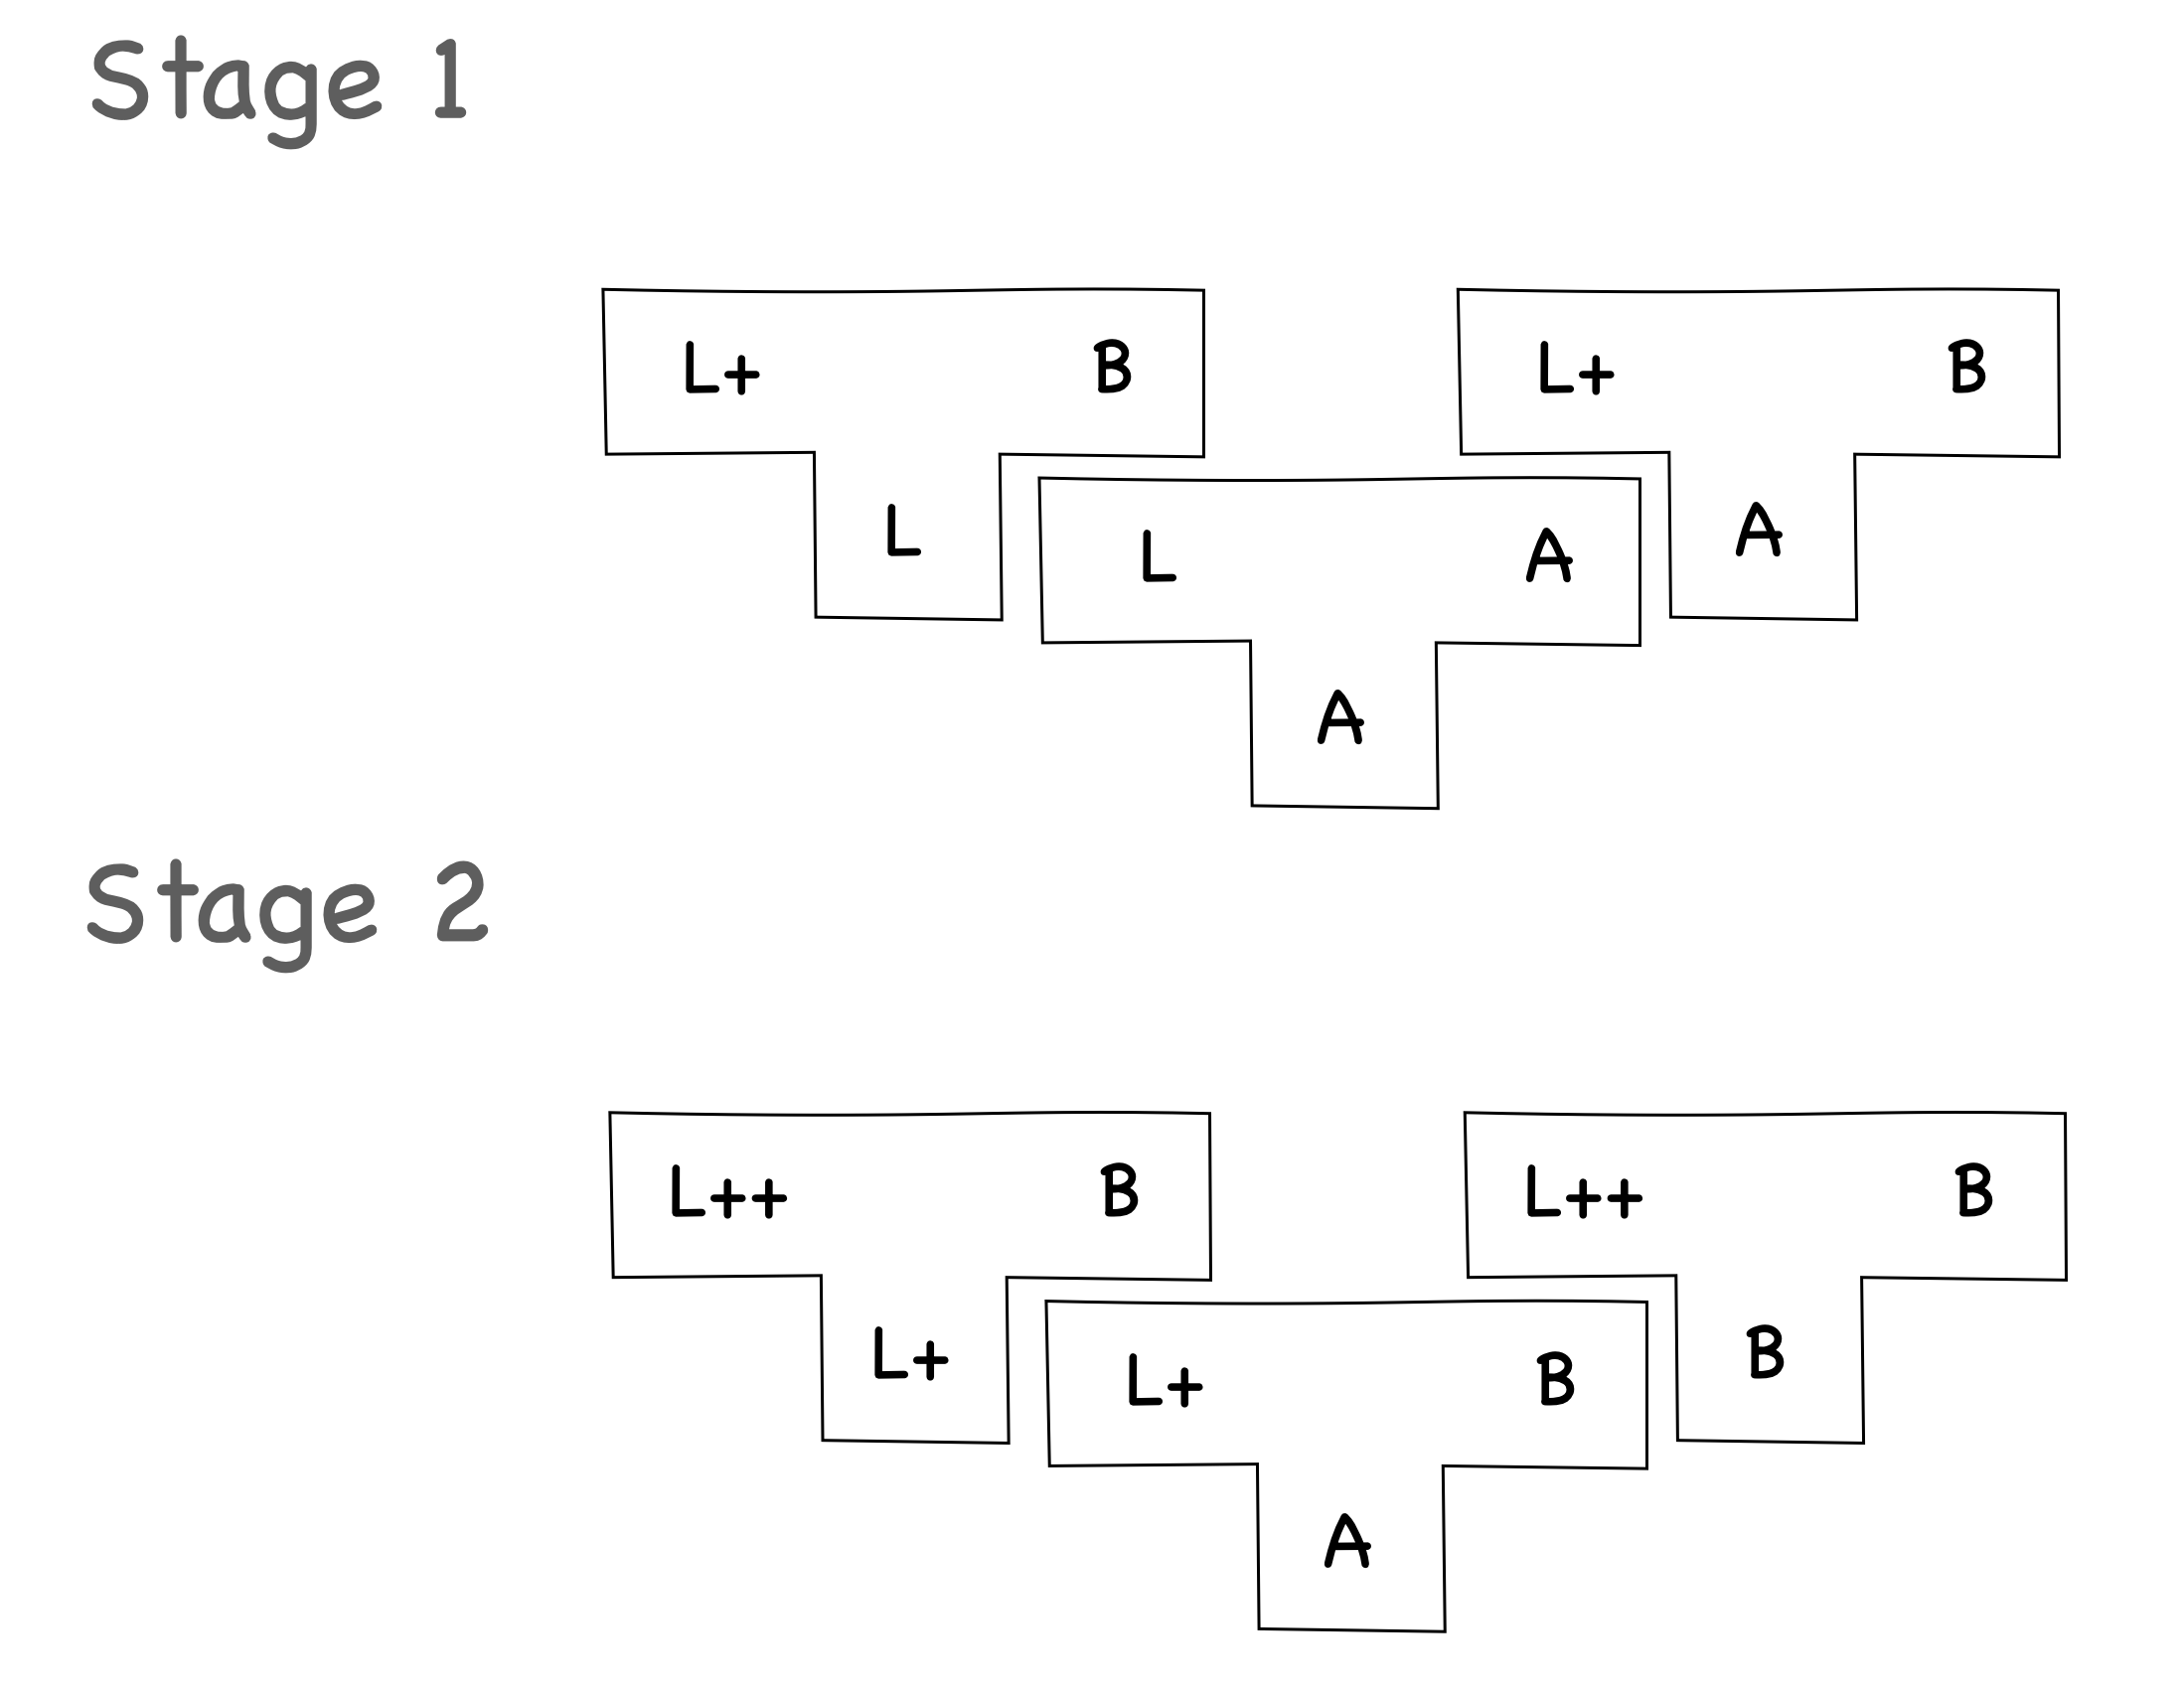
\includegraphics[width=0.8\textwidth]{image/exercise1_1.png}
\end{figure}
